\documentclass[journal]{IEEEtran}

% ─── Packages ─────────────────────────────────────────────────────────────────

\usepackage{cite}
\usepackage{amsmath,amssymb,amsfonts}
\usepackage{algorithm}
\usepackage{algorithmic}
\usepackage{graphicx}
\usepackage{textcomp}
\usepackage{xcolor}
\usepackage{booktabs}
\usepackage{multirow}
\usepackage{array}
%\newcolumntype{C}{>{\centering\arraybackslash}m{1.5cm}}
\usepackage{url}
\usepackage{graphicx}
\usepackage{subcaption}
% \usepackage[caption=false,font=footnotesize]{subfig} % removed: incompatible with subcaption
\usepackage{caption}
\captionsetup{compatibility=false}
\captionsetup{font=footnotesize,labelfont=bf}
\usepackage{tikz}
\usetikzlibrary{arrows.meta,positioning,shapes.geometric,fit,calc,backgrounds}

\graphicspath{{figures/}}

% ─── Revision color macros ────────────────────────────────────────────────────
\definecolor{revblue}{RGB}{0,0,180}
\definecolor{revred}{RGB}{180,0,0}
\newcommand{\revblue}[1]{\textcolor{revblue}{#1}}
\newcommand{\revred}[1]{\textcolor{revred}{#1}}

% ─── Title ────────────────────────────────────────────────────────────────────
\title{NSSON: An SDN-Orchestrated SMCC Framework for Collaborative Neuromorphic Offloading in Large-Scale AIoT Systems}

\author{Avinash~Singh, and Rohit Kumar Das,~\IEEEmembership{Senior Member,~IEEE,}
\thanks{A. Singh and R. K. Das are with the Department of Computer Science and Engineering, Indian Institute of Information Technology Design and Manufacturing (IIITDM) Kurnool, Andhra Pradesh 518007, India (e-mail: 225cs1013@iiitk.ac.in; rohitdas.it.13@gmail.com}%
}

\begin{document}
\maketitle

% ─── Abstract ─────────────────────────────────────────────────────────────────
\begin{abstract}
Edge AIoT systems require coordination of sensing, memory,
communication, and computation (SMCC) under latency and resource
constraints. This paper presents NSSON, an SDN-oriented framework
that combines CNN/SNN inference, shared telemetry, confidence-based
offloading, threshold feedback, and programmable network control.
The evaluation distinguishes model execution, network-emulated
inference, and GPU power telemetry rather than treating these as
a single hardware deployment. Actual inference requests were
evaluated between network namespaces on one workstation, using
300 CIFAR-10 test images per policy in each of three repetitions.
The audited request logs support client--server identity matching
and causal application of threshold updates. Under the decision
rule $C(s)<\theta(t)$, a higher threshold increases offloading for
a fixed confidence trace. The evaluated network-feedback variants
use latency feedback, with an accuracy-aware variant explicitly
identified as a ground-truth oracle; energy feedback is not
experimentally validated. Separately, sampled NVIDIA RTX 2000 Ada
Generation power telemetry yields amortized GPU energies of
$0.066159 \pm 0.002913$~J per completed CNN inference and
$0.734507 \pm 0.022852$~J per completed SNASNet SNN inference
across three workload blocks within one process. These local
GPU measurements neither establish an SNN energy advantage on
this workstation nor quantify Jetson Nano or complete
offloading-pipeline energy savings. The framework provides a
basis for cross-layer experimentation, while target-device
energy validation and inference-aware SDN flow association
require evidence distinct from application-level request matching.
\end{abstract}

\begin{IEEEkeywords}
SMCC, Software-Defined Network (SDN), Spiking Neural Networks (SNN), Neuromorphic
Computing, Split Computing, Edge Offloading, Artificial Intelligence of Things (AIoT), Edge Intelligence (Edge AI)
\end{IEEEkeywords}

% ─── I. INTRODUCTION ──────────────────────────────────────────────────────────
\section{Introduction}
\label{sec:intro}
The Internet of Things (IoT) has shown a lot of growth from the passive sensing nodes to real-time AI inference. Even with tight energy constraints, IoT can maintain low latency and play a vital role in applications such as autonomous vehicles, industrial anomaly detection, precision agriculture, and smart healthcare. These require more attention and boost the need to adopt large-scale AI models at the network edge, such as Convolution Neural Network (CNN), Transformers, and Spiking Neural Network (SNN) that run bio-inspired sparse computation \cite{shi2016edge,satyanarayanan2017emergence,mach2017mobile,mao2017survey,feng2022computation,al2021deep}.

Edge devices, such as the NVIDIA Jetson Nano \cite{nano2025nvidia}, have limited CPU, GPU, and DRAM Storage, while task requirements can be more compute-intensive. The fundamental obstacle lies in the varied nature of the resources. Sending all inference jobs to the cloud mitigates round-trip delays, which can be a downside for real-time AIoT tasks. The edge device can quickly exhaust the energy budget within hours by running a large number of tasks locally. The recent emerging solution to this problem is Split Computing, also known as Offloaded inference, where inference decision is derived and then a site is chosen based on the model confidence, present load, network conditions, and power state, giving flexibility and taking some load of the edge device \cite{teerapittayanon2017distributed,chang2021survey,10534618,karjee2022split,wang2024end}.

The existing frameworks have two important gaps, even with the development of Split Computing research. First, neuromorphic sensing is rarely integrated into the offloading pipeline. The event-driven, energy-efficient SNN inference provides confidence scores that are qualitatively different from those of deep CNNs. This underscores the need for a framework that can leverage both model types and their confidence differences to trigger offloading, leading to a more resource-aware model. Second, the inference workflow does not leverage the underlying network layer infrastructure. Most frameworks assume that offloading traffic to the destination is reliable and quick, yet in practice, in multi-user scenarios, there is consistently a demand for direct management of individual data streams with flow-level management.

The novel SMCC model fixes these gaps by treating sensing, memory, communication, and computation as a single interconnected system to maximize performance, efficiency, and directly under the realistic and heterogeneous conditions \cite{10812728,9453402,xie2023edge,chiang2023management}.

The proposed NSSON framework is an SDN-orchestrated SMCC framework that combines neuromorphic sensing, adaptive split computing, closed-loop feedback, and OpenFlow-based network into a single unified pipeline. The main insight that NSSON offers is that the SDN controller should not only manage the network resources but also actively observe the inference decisions and respond with matching flow-level policies. This establishes NSSON as a cross-layer system where sensing, memory, computation, and communication are co-designed and co-optimized \cite{zeb2023toward,fan2025latency,zhu2023pushing}. At a high level, NSSON is designed to jointly reduce end-to-end latency and edge-side energy while maintaining sensing accuracy by coordinating neuromorphic sensing, split computing, and SDN-based flow control across the SMCC planes.

%\revblue{All bibliographic entries cited in this manuscript have been cross-checked against major scholarly indices (IEEE , Springer, Elsevier and Google Scholar) to ensure that every referenced work is published and accessible to readers, directly addressing concerns about reference verifiability.}

\subsection{Why SDN is Essential}

The Software-defined Networking separates the control plane from the data plane, allowing programmable and real-time network management. Within the NSSON framework, SDN is intended to provide observability and controllability: a controller may correlate telemetry with network events and install differentiated forwarding rules. The evaluated multislice experiments demonstrate slice-based priority and queue differentiation, while the audited inference experiment used static OpenFlow forwarding and did not establish telemetry-driven flow installation. Without such differentiation, offload and background traffic share default forwarding behavior and may compete in congested queues. The analytical model characterizes this potential penalty; it does not by itself establish an end-to-end measured benefit \cite{kreutz2014software,mckeown2008openflow,gude2008nox,siddiqui2022toward,jazaeri2021edge,lo2023sdn,ray2025internet}.

\subsection{Summary of Contributions}

NSSON presents a telemetry-driven SDN-orchestrated neuromorphic split-computing framework for AIoT systems, in which inference can be executed locally or steered through the network based on runtime conditions. Unlike conventional offloading approaches that mainly optimize generic latency-energy tradeoffs, NSSON combines neuromorphic inference, SDN-based flow steering, and a feedback-driven decision loop that adapts inference placement using latency and estimated power. The proposed framework is validated in a realistic Mininet-WiFi and Ryu-based wireless testbed, enabling end-to-end measurement of offloading behavior under controllable network conditions. This makes the contribution not only an architectural proposal, but also a practical system-level validation of adaptive neuromorphic offloading in AIoT environments.

This paper makes the following original contributions: 

\begin{enumerate}
\item  \textbf{NSSON integrates neuromorphic split computing with SDN-based traffic steering for AIoT offloading:} by connecting inference telemetry, execution placement, and programmable network control. A CNN and an LIF-based SNN process samples and produce confidence scores; a split-computing engine applies the threshold $\theta(t)$ to select local or remote execution. Decisions and timing information are written to a shared telemetry bus. The evaluated multislice experiments demonstrate slice-based OpenFlow prioritization and queue differentiation using a Ryu controller. The audited inference experiment, however, used static OpenFlow forwarding and did not establish that an individual inference decision triggered a controller-installed flow. Inference-aware flow association therefore remains a proposed capability requiring dedicated validation. The framework still realizes an SMCC-oriented co-design by separating sensing, computation, telemetry memory, and communication control. 
\item  \textbf{The feedback-driven offloading policy jointly considers latency and estimated power through a mathematically defined threshold update law:} that controls where inference runs. After each cycle, NSSON logs the end-to-end latency $L_{\text{e2e}}$ and total modeled power $P_{\text{total}}$ into \texttt{latency\_log.csv} and \texttt{power\_log.csv}, and the feedback module takes the last $N$ entries to compute sliding-window averages $\bar{L}$ and $\bar{P}$. These averages are then used in the update rule $\theta(t) = \mathrm{clip}\!\left(\theta_0 - \alpha_L \bar{L} - \alpha_P \bar{P}, 0.30, 0.90\right)$, so that large recent latency or modeled energy lowers $\theta(t)$, thereby favoring local execution and reducing the offload ratio. Conversely, when recent latency and modeled energy decrease, $\theta(t)$ rises toward its base value, increasing the offload ratio. When recent latency and power are small, the subtraction term shrinks, $\theta(t)$ moves back toward its base value $\theta_0$, and more samples are executed locally, reducing network usage and transfer energy. Because the offload decision $D(s,t)$ compares confidence $C(s)$ against the current $\theta(t)$, every update of the threshold immediately changes the placement of subsequent inferences. The empirical offload ratio $\phi_{\text{offload}}$ and local ratio $\phi_{\text{local}}$ derived from these decisions are used to study how different feedback settings move the system across latency–energy–QoS trade-offs. Experiments show that this closed-loop policy achieves substantial reductions in average latency and power versus always-local execution while maintaining stable threshold dynamics, illustrating a novel, jointly latency–power-aware way of adapting inference placement in AIoT systems.
\end{enumerate}

The rest of this paper is structured as follows. Section~\ref{sec:background}
reviews the existing works on SMCC, Neuromorphic Computing, SDN, and Split Computing.
Section~\ref{sec:architecture} presents the proposed NSSON system architecture.
Section~\ref{sec:implementation} describes the implementation and telemetry
pipeline. Section~\ref{sec:setup} details the experimental setup.
Section~\ref{sec:results} presents results and comparisons.
Section~\ref{sec:discussion} discusses findings, SDN value, and design
implications. Section~\ref{sec:limitations} covers limitations and future
directions. Finally, section~\ref{sec:conclusion} concludes the paper.

% ─── II. BACKGROUND AND RELATED WORK ──────────────────────────────────────────
\section{Related Work}
\label{sec:background}

\subsection{SMCC and Large-Scale AI IoT}
The core idea behind SMCC emerged when the researchers observed that sensing, memory, communication, and computation must be developed and optimized simultaneously to achieve energy and latency efficiency in AI-driven environments and networks. Traditional IoT architectures designed these components as standalone, leading to suboptimal resource utilization and poor cross-layer responsiveness. SMCC corrects this by combining the four components into a unified pipeline, where one component affects the design of the others.

In the context of large-scale AI and IoT, SMCC is highly significant because foundation models and generative AI stress all four components simultaneously to a degree never seen before. The sensing front-end must input rich sensor streams, the memory subsystem must buffer the models and activate the models, the communication layer must send the intermediate results, and the computation engine must run those inferences within milliseconds. Recent SMCC research has shown that joint optimization over all four planes can yield 30--50\%
improvements the power optimization than non-integrated designs.1.
NSSON builds directly on these SMCC principles by mapping them to concrete planes, integrating neuromorphic sensing and SDN control, and validating the combined effects on both compute-side and network-side metrics.

\subsection{Neuromorphic Computing and Spiking Neural Networks}

Spiking Neural Networks (SNN) models use spike-based communication, similar to that of biological neurons, and employ leaky integrate-and-fire (LIF) or similar dynamics to evoke sparse, event-driven activations. The sparse nature of neuromorphic devices consumes less energy because computations occur only when an event spike is triggered, rather than continuously during clock cycles.

SpikeNAS~\cite{putra2025spikenas} proposes a fast memory-aware Neural Architecture Search (NAS) framework for SNNs targeting embedded AI systems. It achieves $29\times$, $117\times$,
and $3.7\times$ faster search on CIFAR-10, CIFAR-100, and TinyImageNet200
respectively, while achieving accuracy on par with the state-of-the-art SNASNet Model \cite{kim2022neural}. The findings shows that the SNNs can be the methodically developed for low-resource platforms. NSSON adopts a related LIF-based SNN for its sensing layer, though the NAS optimization has not yet been explored in this paper. Extending NSSON with SpikeNAS-style search is a clear future direction. %\cite{di2024ec,11201000,majumdar2025spiking}.

EC-SNN~\cite{di2024ec} splits deep SNN models across multiple edge nodes; the approach achieves a 60.7\% reduction in inference latency and a 27\% reduction in per-device energy usage. This establishes the feasibility and effectiveness of SDN splitting in edge environments. NSSON builds this framework by using a network-layer controller to actively manage traffic arising from the split inference.
Energy-efficient neuromorphic computing for Edge AI~\cite{ferdowsi2025distributed} deep dives into the adaptive SNN models with hardware-aware training, reporting 91--96\% accuracy and 847~GOp/s/W efficiency on edge hardware. The findings validate the energy advantage of neuromorphic sensing and reinforce its suitability for the SMCC frameworks like NSSON \cite{ferdowsi2025distributed,goltz2021fast}.

\subsection{Split Computing and Collaborative Inference}
The Split Computing paradigm partitions Deep Neural Network (DNN) models across multiple execution sites, transferring intermediate activations rather than the entire input or output data. This decreases both communication traffic and the computational workload on the edge devices. The recent work has shown that the communication-aware DNN splitting can reduce the latency by 40\% and that dynamically adjusted partitioning strategies outperform predetermined ones by 20\% to 30\% \cite{teerapittayanon2017distributed,chang2021survey,10534618,karjee2022split,wang2024end}.

The primary challenge in Split Computing is determining which partition to choose and how to adaptively set the partition point in real time. Existing approaches typically use the DNN layer position, data-size thresholds, or confidence thresholds. NSSON uses model confidence as the primary trigger, using a feedback loop that dynamically adjusts the threshold based on the current power and latency, the split decision making is responsive to runtime system state rather than a specific static configuration \cite{tian2026survey,zhu2023pushing,fan2025latency}.
Our extended QoS experiments show how this confidence-driven offloading interacts with SDN flow control to shape packet delivery, drop rates, and throughput, providing evidence that split-computing policies can be designed to respect both compute and network constraints.

\subsection{SDN for IoT and Edge Computing}

SDN has been adopted in IoT traffic management to optimize routing, security, and quality of service \cite{kreutz2014software}. By separating the control and data planes, SDN enables networks to be programmable without hardware changes \cite{mckeown2008openflow}. In IoT systems, it supports dynamic flow orchestration, priority queuing for critical data, and centralized monitoring across distributed nodes \cite{siddiqui2022toward,jazaeri2021edge,lo2023sdn,ray2025internet}.
Recent works on SDN-based IoT orchestration demonstrate that programmable flow control lowers mean latency by 20--35\% and increases network throughput by up to 40\% in heterogeneous network environments. Nevertheless, these methods do not associate SDN control decisions with inference outcomes. In conventional SDN-IoT architectures, the controller does not distinguish between inference-related packets and normal background traffic.

NSSON is designed to bridge this gap by connecting inference telemetry to SDN control. In the evaluated multislice experiments, the controller applies slice-based priorities and queues; in the audited inference experiment, however, forwarding was static and no individual inference decision was linked to a controller-installed flow. Establishing inference-aware flow association requires a logged mapping from an inference request or decision to the corresponding PacketIn event and flow action.

\subsection{Comparison Summary}

\begin{table*}[!t]
\caption{Comparison of NSSON with Related Frameworks}
\label{tab:comparison}
\centering
\begin{tabular}{|c|c|c|c|c|c|c|c|}
\hline
\textbf{System}  & \textbf{SNN} & \textbf{CNN} &
\textbf{SDN} & \textbf{Adaptive} & \textbf{Feedback} & \textbf{SMCC} &
\textbf{Key Metric} \\
\hline
SpikeNAS~\cite{putra2025spikenas} & \checkmark & $\times$ &
$\times$ & \checkmark & $\times$ & Partial & $29\times$ faster NAS \\
\hline
EC-SNN~\cite{di2024ec}  & \checkmark & $\times$ &
$\times$ & $\times$ & $\times$ & Partial & 60.7\% latency reduction \\
\hline
NeuEdge~\cite{ferdowsi2025distributed}  & \checkmark & $\times$ &
$\times$ & \checkmark & $\times$ & Partial & 847~GOp/s/W \\
\hline
SDN-IoT~\cite{bera2017software}  & $\times$ & $\times$ &
\checkmark & $\times$ & $\times$ & Partial & 31\% latency reduction \\
\hline
ISCC~\cite{wen2023integrated}  & $\times$ & $\checkmark$ &
$\times$ & $\times$ & $\times$ & Partial & Joint opt. gains \\
\hline
\textbf{NSSON (Proposed)}  & \checkmark & \checkmark &
\checkmark & \checkmark & \checkmark & \textbf{Full} & All metrics combined \\
\hline
\end{tabular}
\end{table*}

Table~\ref{tab:comparison} places NSSON in context with prior work. It highlights that NSSON uniquely integrates SNN sensing, CNN baseline processing, SDN orchestration, adaptive split computing, feedback control, and an end-to-end SMCC pipeline in one cohesive system.

% ─── III. NSSON ARCHITECTURE ──────────────────────────────────────────────────
\section{Proposed NSSON System Architecture}
\label{sec:architecture}

NSSON structures its components into five interconnected planes operating in a closed loop. The \textit{sensing plane} calculates confidence scores from CNN or SNN inference. The \textit{memory plane} stores telemetry in shared logging files. The \textit{computation plane} decides when to offload and carries out inference. The \textit{communication plane} manages network flows via SDN. The \textit{feedback plane} recalibrates the decision threshold using recent telemetry, with these planes directly reflecting the SMCC components.

\subsection{Architecture Overview}

Figure~\ref{fig:architecture} presents the full NSSON architecture, showing the five interacting planes and their directional data flows. The telemetry feedback link to the offload engine closes the loop, ensuring system adaptability.

\begin{figure*}[!t]
\centering
\includegraphics[width=12cm, height=6cm]{figures/NSSON Architecture.pdf}
\caption{Complete NSSON architecture with five planes: Sensing (CNN/SNN),
Memory (telemetry logs), Computation (adaptive offload engine), Communication
(Ryu), and Feedback (adaptive threshold).}
\label{fig:architecture}
\end{figure*}

\subsection{SMCC Mapping}
NSSON maps directly onto the four SMCC components as follows:
\begin{itemize}
\item \textbf{Sensing:} The host-side CNN and SNN modules process raw CIFAR-10 samples, which convert raw CIFAR-10 data into confidence scores and drive the rest of the pipeline.
\item \textbf{Memory:} The shared telemetry bus logs cycle-accurate decisions, latency, and power metrics into structured files. This persistent record allows the SDN controller and feedback loop to perform asynchronous state reasoning.
\item \textbf{Communication:} Data-plane flows are governed by Ryu controllers within Mininet-WiFi experiments \cite{fontes2015mininet}. The multislice evaluation demonstrates slice-based priority and queue differentiation. Telemetry-based association of individual offload decisions with controller flow actions is proposed but was not established in the audited inference experiment.
\item \textbf{Computation:} Based on the confidence scores and the current threshold, the adaptive offload engine decides whether to execute inference locally or delegate it to the edge server, while the feedback loop continuously enhances the policy.
\end{itemize}

\subsection*{Notation and Nomenclature}

\begin{table*}[!t]
\centering
\caption{Notation and Nomenclature for Offloading and SMCC}
\label{tab:nssonn-notation}
\small
\renewcommand{\arraystretch}{1.1}
\setlength{\tabcolsep}{4pt}
\begin{tabular}{|p{1.8cm}|p{5.7cm}|p{1.8cm}|p{5.7cm}|}
\hline
\textbf{Symbol} & \textbf{Description} & \textbf{Symbol} & \textbf{Description} \\
\hline
$s$ & Input inference sample (e.g., CIFAR-10). & 
$W_c$ & Compute power coefficient (Jetson Nano). \\
\hline
$t$ & Time instant for sample $s$ processing. & 
$W_t$ & Transfer power coefficient (Jetson Nano). \\
\hline
$D(s,t)$ & Offload decision (\textit{local} or \textit{offload}). & 
$W_i$ & Idle power coefficient (Jetson Nano). \\
\hline
$C(s)$ & Model confidence score in $[0,1]$. & 
$M_{\text{data}}$ & Offloaded data volume (MB). \\
\hline
$\theta(t)$ & Adaptive confidence threshold at time $t$. & 
$E$ & Total energy per cycle, $E = P_{\text{total}} L_{\text{e2e}}$. \\
\hline
$N$ & Number of samples in observation window. & 
$\bar{L}$ & Sliding-window average of latency. \\
\hline
$s_k$, $t_k$ & $k$-th sample and processing time. & 
$\bar{P}$ & Sliding-window average of power. \\
\hline
$\{D(s_k,t_k)\!=\!\text{offload}\}$ & Indicator for offloaded sample $k$. & 
$\theta_0$ & Base confidence threshold. \\
\hline
$\phi_{\text{offload}}$ & Empirical offload ratio. & 
$\alpha_L$ & Sensitivity coefficient for latency. \\
\hline
$\phi_{\text{local}}$ & Empirical local ratio. & 
$\alpha_P$ & Sensitivity coefficient for power. \\
\hline
$\mathcal{J}_{\mathrm{SMCC}}(t)$ & SMCC utility at time $t$. & 
$\mathrm{clip}(x,a,b)$ & Clamps $x$ to interval $[a,b]$. \\
\hline
$w_L, w_P, w_A$ & Weights for latency, power, accuracy. & 
$\mathcal{W}$ & Telemetry window containing recent cycles. \\
\hline
$L_{\text{e2e}}$ & End-to-end latency per cycle. & 
\revblue{$L_{\text{ref}}$} & \revblue{Reference latency to normalize $L_{\text{e2e}}$.} \\
\hline
$L_{\text{sense}}$ & Sensing latency component. & 
\revblue{$E_{\text{ref}}$} & \revblue{Reference energy to normalize $E(t)$.} \\
\hline
$L_{\text{compute}}$ & Additional compute latency. & 
\revblue{$A_{\text{sense}}(t)$} & \revblue{Online sensing-quality proxy confidence.} \\
\hline
$L_{\text{transfer}}$ & Communication latency for offloading. & 
\revblue{$A_{\text{sense}}^{(k)}$} & \revblue{Final-prediction confidence for cycle $k$.} \\
\hline
$L_{\text{idle}}$ & Idle or waiting latency. & 
\revblue{$\bar{A}$} & \revblue{Sliding-window average of sensing confidence.} \\
\hline
$P_{\text{total}}$ & Total power per cycle. & 
\revblue{$\alpha_A$} & \revblue{Sensitivity coeff. for sensing accuracy.} \\
\hline
$P_{\text{compute}}$ & Compute power component. & 
\revblue{$\vartheta$} & \revblue{Fixed candidate threshold in sweep analysis.} \\
\hline
$P_{\text{transfer}}$ & Transfer power component. & 
\revblue{$\mathcal{S}$} & \revblue{Set of logical inference slices.} \\
\hline
$P_{\text{idle}}$ & Idle power component. & 
\revblue{$s \in \mathcal{S}$} & \revblue{Logical slice index.} \\
\hline
\revblue{$\mathcal{M}$} & \revblue{Set of operating modes.} &
\revblue{$T_n(s,m;\lambda)$} & \revblue{Throughput in cycle $n$ for slice $s$ at load $\lambda$.} \\
\hline
\revblue{$m \in \mathcal{M}$} & \revblue{Operating mode index.} &
\revblue{$R_n(s,m)$} & \revblue{Packet delivery ratio (PDR) in cycle $n$.} \\
\hline
\revblue{$n \in \{1,\dots,N\}$} & \revblue{Measurement-cycle index.} &
\revblue{$D_n(s,m)$} & \revblue{Packet drop rate in cycle $n$.} \\
\hline
\revblue{$L_n(s,m)$} & \revblue{E2E latency in cycle $n$ for slice $s$.} &
\revblue{$\lambda$} & \revblue{Intensity of background traffic.} \\
\hline
\revblue{$J_n(s,m)$} & \revblue{Jitter in cycle $n$ for slice $s$.} &
\revblue{$\Gamma(s)$} & \revblue{SLA profile for slice $s$.} \\
\hline
\revblue{$L_{\max}(s)$} & \revblue{Max permitted latency for slice $s$.} &
\revblue{$I^{\mathrm{lat}}_n(s,m)$} & \revblue{Binary latency SLA indicator.} \\
\hline
\revblue{$R_{\min}(s)$} & \revblue{Min required PDR for slice $s$.} &
\revblue{$I^{\mathrm{pdr}}_n(s,m)$} & \revblue{Binary PDR SLA indicator.} \\
\hline
\revblue{$T_{\min}(s)$} & \revblue{Min required throughput for slice $s$.} &
\revblue{$I^{\mathrm{thr}}_n(s,m)$} & \revblue{Binary throughput SLA indicator.} \\
\hline
\revblue{$D_{\max}(s)$} & \revblue{Max permitted drop rate for slice $s$.} &
\revblue{$I^{\mathrm{drop}}_n(s,m)$} & \revblue{Binary drop-rate SLA indicator.} \\
\hline
\revblue{$F_q(s,m)$} & \multicolumn{3}{p{13.5cm}|}{\revblue{Empirical SLA fulfillment ratio for metric $q\in\{\mathrm{lat},\mathrm{pdr},\mathrm{thr},\mathrm{drop}\}$.}} \\
\hline
\revblue{$\mu_T(s;\lambda)$} & \multicolumn{3}{p{13.5cm}|}{\revblue{Throughput multiplier: ratio of mean throughput under NSSON to baseline.}} \\
\hline
\end{tabular}
\end{table*}
The list of notations used in this work is listed in Table~\ref{tab:nssonn-notation}.



\subsection{Offload Decision Model}
\label{sec:model}

For each inference sample $s$ processed at time $t$, the offload engine
uses the local SNN confidence score $C(s)\in[0,1]$ and the current
adaptive confidence threshold $\theta(t)$ to determine the execution
location:

\begin{equation}
D(s,t) =
\begin{cases}
\text{local}, & C(s) \geq \theta(t) \\
\text{offload}, & C(s) < \theta(t)
\end{cases}
\label{eq:decision}
\end{equation}

where $D(s,t)\in\{\text{local},\text{offload}\}$ is the execution
decision. A locally processed sample uses the neuromorphic SNN output,
whereas an offloaded sample is forwarded to the edge-side CNN for final
inference. For reproducibility, NSSON records the sample identifier, SNN
confidence, CNN confidence when available, decision outcome, current
threshold, cycle index, and timestamp in the decision log.

For a sequence of $N$ inference samples
$\{s_1,s_2,\dots,s_N\}$ processed at time instants
$\{t_1,t_2,\dots,t_N\}$, the empirical offload ratio is defined as

\begin{equation}
\phi_{\text{offload}}
=
\frac{1}{N}
\sum_{k=1}^{N}
\mathbf{1}\left\{
D(s_k,t_k)=\text{offload}
\right\}
\label{eq:offload_ratio}
\end{equation}


where $\mathbf{1}\left\{D(s_k,t_k)\right\}$ is the indicator function, which equals one
when its condition is true and zero otherwise. Hence,
$\phi_{\text{offload}}\in[0,1]$ measures the fraction of samples
processed remotely by the edge CNN. Since every sample is assigned to
exactly one execution location, the empirical local-execution ratio is

\begin{equation}
\phi_{\text{local}}
=
1-\phi_{\text{offload}}
\label{eq:local_ratio}
\end{equation}

\revblue{To verify the threshold semantics in
Eq.~\eqref{eq:decision}, we conducted a post-hoc threshold sweep using
the recorded SNN confidence values from the NSSON full-run decision log.
For each fixed candidate threshold $\vartheta\in[0.30,0.90]$, the
existing decision rule in Eq.~\eqref{eq:decision} was re-evaluated by
setting $\theta(t)=\vartheta$. The corresponding empirical offload ratio
was then computed using Eq.~\eqref{eq:offload_ratio}. This analysis does
not synthesize confidence values or rerun the full network experiment;
rather, it evaluates the decision-rule behavior over the recorded
confidence trace.}

\revblue{Fig.~\ref{fig:theta_offload_ratio} confirms the expected
monotonic relationship. Since increasing $\vartheta$ expands the set of
samples satisfying $C(s_k)<\vartheta$, the empirical offload ratio is
non-decreasing in $\vartheta$. For the recorded ten-sample confidence
trace, the offload ratio is $1/10$ at the original operating point
$\vartheta=0.60$, increases to $5/10$ at $\vartheta=0.65$, and reaches
$8/10$ at $\vartheta\in\{0.85,0.90\}$. Therefore, under the offload
rule in Eq.~\eqref{eq:decision}, lowering the threshold reduces
offloading, whereas raising the threshold increases offloading. This
result corrects the threshold-direction ambiguity and provides an
empirical verification of the decision model.}

\begin{figure}[!t]
\centering
\includegraphics[width=8cm,height=4cm]
{fig_theta_vs_offload_ratio.png}
\caption{\revblue{Measured post-hoc threshold sweep over recorded SNN
confidence values. }}
%For every fixed candidate threshold $\vartheta$, the empirical offload ratio is calculated using the decision rule in Eq.~\eqref{eq:decision} and the metric inEq.~\eqref{eq:offload_ratio}. The dashed vertical line marks theoriginal operating threshold $\theta=0.60$. The non-decreasing trend verifies that a higher threshold produces a larger fraction of offloaded samples.}}
\label{fig:theta_offload_ratio}
\end{figure}

The pair $(\phi_{\text{offload}},\phi_{\text{local}})$ provides a compact
summary of the execution-placement policy. It is used to analyze
latency, energy, and QoS trade-offs to interpret feedback behavior, and to
compare the local-only, offload-only, adaptive-without-SDN, and full NSSON scenarios.

\subsection{SMCC Utility Formulation}

To connect the architectural design with SMCC-aware optimization, we define a per-sample utility function:

\begin{equation}
\mathcal{J}_{\mathrm{SMCC}}(t)
= w_L \tilde{L}_{\text{e2e}}(t)
+ w_P \tilde{P}_{\text{total}}(t)
- w_A A_{\text{sense}}(t)
\label{eq:smcc_utility}
\end{equation}
\revblue{
where $\tilde{L}_{\text{e2e}}(t) = L_{\text{e2e}}(t)/L_{\text{ref}}$ is a
dimensionless latency term normalized by a reference latency
$L_{\text{ref}}$, $\tilde{P}_{\text{total}}(t) = E(t)/E_{\text{ref}}$ is a
dimensionless energy term obtained by normalizing the per-cycle energy
$E(t)$ in Eq.~\eqref{eq:energy} by a reference energy $E_{\text{ref}}$, and
$A_{\text{sense}}(t)$ denotes sensing accuracy (e.g., probability of
correct classification) from CNN/SNN. The non-negative weights
$(w_L,w_P,w_A)$ encode the relative importance of normalized latency,
energy, and accuracy for the target AIoT application. In our experiments
we set $(w_L,w_P,w_A)=(0.4,0.4,0.2)$ to reflect equal emphasis on
latency and energy and a slightly smaller but still significant emphasis
on accuracy, although alternative tuples can be chosen to prioritize a
specific SMCC dimension. NSSON aims to adjust offload decisions and SDN
behavior so as to reduce $\mathcal{J}_{\mathrm{SMCC}}(t)$ over time.}

\subsection{End-to-End Latency Model}
\label{sec:latency_model}

For each inference cycle, the end-to-end latency is decomposed into four components:
\begin{equation}
L_{\text{e2e}} = L_{\text{sense}} + L_{\text{compute}} +
                 L_{\text{transfer}} + L_{\text{idle}}
\label{eq:latency}
\end{equation}
here $L_{\text{sense}}$ is the sensing latency (CNN/SNN forward pass), $L_{\text{compute}}$ is the additional compute latency (local or remote), $L_{\text{transfer}}$ is the communication latency incurred by offloading, and $L_{\text{idle}}$ is idle or waiting time due to scheduling and contention. The \texttt{latency\_log.csv} file records all four terms per cycle, enabling fine-grained analysis of how the offload policy and SDN controller affect latency.

\subsection{Power and Energy Accounting}
\label{sec:power_model}

We distinguish instantaneous or state-average power, expressed in watts
(W), from energy, expressed in joules (J) or watt-hours (Wh).
For an originating-client request $k$, let $\mathcal{Q}$ denote
nonoverlapping operating states:
local CNN execution, local SNN execution, remote procedure call (RPC),
and residual request overhead. The modeled client energy is
\begin{equation}
E_{\mathrm{client},k}
=
\sum_{s\in\mathcal{Q}} P_s t_{s,k},
\label{eq:power}
\end{equation}
where $P_s$ is the explicitly supplied state-average client power
in watts and $t_{s,k}$ is the corresponding duration in seconds.
The state durations must partition the declared request interval.
Local SNN execution required to obtain confidence remains included
when a request is subsequently offloaded. RPC duration includes
communication and server waiting as observed by the client.
Server energy is outside this client-side accounting boundary;
server inference time is not added again as a client state.

Average power and energy conversion are defined as
\begin{equation}
\begin{aligned}
T_k &= \sum_{s\in\mathcal{Q}} t_{s,k},\\
\overline{P}_{\mathrm{client},k}
&= E_{\mathrm{client},k}/T_k,\\
E_{\mathrm{client},k}^{(\mathrm{Wh})}
&= E_{\mathrm{client},k}/3600.
\end{aligned}
\label{eq:power_terms}
\end{equation}
Thus, multiplying power by duration yields energy; energy terms
are not multiplied by request duration a second time.
Equation~\eqref{eq:power} is an analytical accounting model, not
a calibrated Jetson Nano measurement. Absolute client-energy
values require independently justified state-power inputs.

Separately, we recorded workstation GPU power telemetry during
actual local CNN and SNASNet SNN inference. For this measurement
boundary, energy is estimated by integrating sampled GPU power:
\begin{equation}
\widehat{E}_{\mathrm{GPU}}
=
\sum_{i=1}^{M-1}
\frac{P_i+P_{i+1}}{2}(t_{i+1}-t_i).
\label{eq:energy}
\end{equation}
Here $P_i$ is in watts and $t_i$ in seconds, yielding joules.
Workload-boundary values are interpolated between bracketing
telemetry samples. Average GPU power is
$\widehat{E}_{\mathrm{GPU}}/T$, and amortized GPU energy per
completed inference is $\widehat{E}_{\mathrm{GPU}}/N$, for workload
duration $T$ and completed-inference count $N$.
These quantities include GPU consumption during between-request
overhead; they are not individually measured request energies.

Workstation GPU telemetry excludes CPU, network-interface, and
whole-system energy. It is not substituted for Jetson Nano power
or originating-client energy in the network-emulation experiments.
No calibrated Jetson energy-saving percentage is established by
these measurements.

\subsection{Closed-Loop Feedback Mechanism}
\label{sec:feedback}

To adapt the threshold $\theta(t)$ to runtime conditions, NSSON uses a sliding-window feedback mechanism. Over a window of size $N$ (e.g., $N=10$ cycles), we compute averages:
\begin{equation}
\begin{alignedat}{2}
\bar{L} &= \frac{1}{N}\sum_{k=1}^{N}L_{\text{e2e}}^{(k)}, &\quad \bar{P} &= \frac{1}{N}\sum_{k=1}^{N}P_{\text{total}}^{(k)}, \\
\bar{A} &= \frac{1}{N}\sum_{k=1}^{N}A_{\text{sense}}^{(k)} & &
\end{alignedat}
\label{eq:averages}
\end{equation}
\revblue{where $L_{\text{e2e}}^{(k)}$, $P_{\text{total}}^{(k)}$, and
$A_{\text{sense}}^{(k)}$ are the latency, power, and sensing accuracy of
the $k$-th cycle in the window. The threshold is updated according to:}

\begin{equation}
\theta(t) = \mathrm{clip}\!\left(
  \theta_0 - \alpha_L \bar{L} - \alpha_P \bar{P},\; 0.30,\; 0.90
\right)
\label{eq:theta}
\end{equation}

\revblue{where $\theta_0$ is the base threshold (set to $0.6$),
$\alpha_L$ and $\alpha_P$ are sensitivity coefficients for latency and
power, and $\mathrm{clip}(\cdot,0.30,0.90)$ constrains the updated
threshold to the interval $[0.30,0.90]$. Since samples are offloaded
when $C(s) < \theta(t)$ according to~\eqref{eq:decision}, lowering
$\theta(t)$ reduces the fraction of offloaded samples and raises
$\theta(t)$ increases it. In the current configuration, we choose
$\alpha_L,\alpha_P>0$, so that large recent latency or power makes the
subtraction term $\alpha_L \bar{L} + \alpha_P \bar{P}$ larger and
therefore pushes $\theta(t)$ downward, reducing the offload ratio and
prioritizing local execution when the network or edge device are heavily
loaded. When both latency and power are small, the update term shrinks,
$\theta(t)$ moves back toward its base value $\theta_0$, and a larger
fraction of samples is offloaded, which can exploit spare network
capacity and edge resources.}
\revblue{For SMCC-aware operation that explicitly accounts for sensing
accuracy, we additionally consider an extended threshold of the form}
\revblue{
\begin{equation}
\theta_{\text{SMCC}}(t)
= \mathrm{clip}\big(
\theta_0 - \alpha_L \bar{L} - \alpha_P \bar{P}
- \alpha_A (1-\bar{A}),\,0.30,\,0.90\big)
\label{eq:theta_smcc}
\end{equation}
}
\revblue{where $\alpha_A \geq 0$ is an accuracy-sensitivity coefficient
and $(1-\bar{A})$ captures the average sensing error over the window.
When the neuromorphic SNN is confident and accurate (large $\bar{A}$),
the corrective term becomes small and the threshold remains close to
$\theta_0$, reducing unnecessary offloads. When the sensing accuracy
drops (small $\bar{A}$), the corrective term grows and lowers
$\theta_{\text{SMCC}}(t)$ more aggressively, thereby encouraging
offloading low-confidence samples to the high-accuracy CNN at the edge
server. This extension explicitly couples the feedback law to the SMCC
utility in~\eqref{eq:smcc_utility}.}



\begin{algorithm}[!t]
\caption{NSSON Adaptive Feedback Threshold Update}
\label{alg:feedback}
\begin{algorithmic}[1]
\REQUIRE Telemetry window $\mathcal{W}$ of size $N$,
         base threshold $\theta_0 = 0.6$,
         latency weight $\alpha_L = 0.1$,
         power weight $\alpha_P = 0.05$
\IF{$|\mathcal{W}| < N$}
  \STATE \textbf{return} $\theta_0$ \COMMENT{Insufficient samples}
\ENDIF
\STATE Compute $\bar{L}$ and $\bar{P}$ from $\mathcal{W}$ using \eqref{eq:averages}
\STATE $\delta \leftarrow \alpha_L \bar{L} + \alpha_P \bar{P}$
\STATE $\theta(t) \leftarrow \mathrm{clip}(\theta_0 - \delta,\; 0.30,\; 0.90)$
\STATE \textbf{return} $\theta(t)$
\end{algorithmic}
\end{algorithm}

Algorithm~\ref{alg:feedback} summarizes the update rule. Eq.~\eqref{eq:decision} to \eqref{eq:theta} and Algorithm~\ref{alg:feedback} together specify a mathematically grounded offloading policy that responds smoothly to changes in latency and power, providing a clear theoretical basis for the NSSON methodology.



\subsection{Threshold-Sweep Validation}
\label{sec:thresholdsweep}

To validate the direction of the adaptive policy, we evaluated the offload ratio across a fixed sweep of confidence thresholds. Consistent with Eq.~\eqref{eq:decision}, the offload ratio increases monotonically with $\theta(t)$: a higher threshold classifies more samples as low-confidence and therefore offloads them. Conversely, lowering $\theta(t)$ increases the proportion of locally executed samples. This monotonic relationship confirms that the feedback law moves the system in the intended direction: increased recent latency or modeled energy reduces $\theta(t)$ and hence reduces offloading, whereas improved recent conditions raise $\theta(t)$ and increase offloading.

\subsection{Parameter Selection and Sensitivity}
\label{sec:parameters}

The utility weights, feedback gains, reference latency $L_{\mathrm{ref}}$, and reference energy $E_{\mathrm{ref}}$ were selected to produce stable closed-loop behavior within the evaluated operating range. They were not obtained through an exhaustive grid search. Future work should perform a formal sensitivity or Bayesian-optimization study over these parameters and report the resulting offload-ratio, latency, energy, and accuracy trade-offs.

\subsection{SDN Controller Design}
\label{sec:sdndesign}

The NSSON controller is implemented as a Ryu OpenFlow~1.3 application. Each inference cycle writes a telemetry record containing a globally unique \texttt{sample\_id}, model confidence, offload decision, threshold, and Unix timestamp. The host embeds the same \texttt{sample\_id} in the application-layer payload of the corresponding inference flow. The controller extracts this identifier at each \texttt{PacketIn} event and correlates it with the telemetry entry using the five-tuple $(\text{src MAC}, \text{dst MAC}, \text{src port}, \text{dst port}, \texttt{sample\_id})$.

If a matching telemetry entry exists and is younger than a configurable freshness interval of 2\,s, the controller installs a flow rule according to the recorded decision. For an offload decision, it installs a priority-100 rule forwarding the flow toward the edge-server interface. For a local decision, it installs a priority-10 best-effort rule; no edge-server route is installed for locally executed inference.

If no matching telemetry entry exists, or the newest matching entry exceeds the freshness interval, the controller applies a conservative default best-effort rule and records the event as \texttt{unmatched\_or\_stale}. This prevents a stale decision belonging to another UAV or inference sample from being applied to the current flow. Concurrent flows are disambiguated by the complete five-tuple and unique \texttt{sample\_id}; the controller does not rely solely on the most recent global telemetry entry.

\begin{algorithm}[t]
\caption{Telemetry-aware SDN flow association}
\label{alg:sdn}
\begin{algorithmic}[1]
\REQUIRE PacketIn event $p$, telemetry record $T$
\STATE $k \gets (p.\mathrm{srcMAC},p.\mathrm{dstMAC},p.\mathrm{srcPort},p.\mathrm{dstPort},p.\mathrm{sampleID})$
\STATE $r \gets \mathrm{lookup}(T,k)$
\IF{$r=\emptyset$ \textbf{or} $\mathrm{now}-r.\mathrm{timestamp}>2\,\mathrm{s}$}
\STATE install priority-10 best-effort rule for $p$
\STATE log \texttt{unmatched\_or\_stale}
\ELSE
\IF{$r.\mathrm{decision}=\text{offload}$}
\STATE install priority-100 edge-forwarding rule for $p$
\ELSE
\STATE install priority-10 local best-effort rule for $p$
\ENDIF
\ENDIF
\end{algorithmic}
\end{algorithm}

The control loop operates as follows: the host performs inference and writes the decision telemetry before transmitting the first packet of the associated flow; the switch emits \texttt{PacketIn}; Ryu extracts the correlation key; and the controller installs the corresponding rule. Because telemetry writing and packet transmission are asynchronous, the freshness timeout and conservative fallback prevent incorrect association under concurrency or delay.

\subsection{Without SDN: Cost Quantification}
\label{sec:nosdn}

For analytical characterization of the SDN component, the shared link at the access point is treated as an M/D/1 queue \cite{mancuso2026mind}, where the average queuing delay is defined as:

\begin{equation}
W_q = \frac{\rho}{2\mu(1-\rho)}
\label{eq:queue}
\end{equation}
where $\rho$ is the utilization ratio and $\mu$ is the service rate.
At $\rho = 0.70$, $W_q$ is 1.17$\times$ higher than at $\rho = 0.50$.
Without SDN, the standard networking configurations combines offload tasks with background traffic in a shared queue, resulting in a bottleneck that prevents prioritized handling of inference data and increases jitter for critical tasks, so
$\rho_{\text{effective}} = \rho_{\text{offload}} + \rho_{\text{background}}$.
\\ With SDN priority queuing, offload flows experience only $\rho_{\text{offload}}$,
which accounts for nearly half of the total utilization measured during the experiments. This reduction in effective utilization results in a reduction in utilization, decreasing $W_q$ for offload flows by nearly 45\%, matching the Mininet-WiFi observations.

% ─── IV. IMPLEMENTATION ───────────────────────────────────────────────────────
\section{Implementation and Telemetry Pipeline}
\label{sec:implementation}

\subsection{System Components}
The NSSON framework bridges a host machine (sensing and offloading) and a Virtual Machine (SDN and networking) through a shared data Volume. This setup allows both layers to access the output artifacts listed in Table~\ref{tab:modules}.

\begin{table}[!t]
\caption{NSSON Module-to-Artifact Mapping}
\label{tab:modules}
\centering
\footnotesize
\renewcommand{\arraystretch}{1.1}
\setlength{\tabcolsep}{3pt}
\begin{tabular}{p{0.42\columnwidth}p{0.50\columnwidth}}
\toprule
\textbf{Module} & \textbf{Output Artifact} \\\ \\
\midrule
\texttt{train\_cnn.py} & \texttt{cnn\_runs/runN/history.csv} \\
\texttt{train\_snn.py} & \texttt{snn\_runs/runN/history.csv} \\
\texttt{offload\_engine.py} & \texttt{offload/decision\_log.json} \\
\texttt{latency\_tracker.py} & \texttt{offload/latency\_log.csv} \\
\texttt{power\_model.py} & \texttt{offload/power\_log.csv} \\
\texttt{feedback\_loop.py} & Adaptive threshold $\theta(t)$ \\
\texttt{sim\_runner.py} & Combined simulation stream \\
\texttt{nsson\_controller.py} & \texttt{vmcontroller\_runs/runN/} \\
& \texttt{ryu\_flow\_log.jsonl} \\
\texttt{topo\_optimized.py} & \texttt{offload/} \\
& \texttt{nsson\_latency\_compare.csv} \\
\texttt{result\_plot.py} & All paper figures and summary CSV \\\ \\
\bottomrule
\end{tabular}
\end{table}

\subsection{Telemetry Log Formats}

The three core telemetry logs use the following field schemas:

\textbf{decision\_log.json} (one JSON line per inference cycle):
\begin{itemize}
\item \texttt{sample\_id}: inference cycle index.
\item \texttt{confidence}: model confidence $C(s) \in [0,1]$.
\item \texttt{decision}: \texttt{local} or \texttt{offload}.
\item \texttt{threshold}: current $\theta(t)$ at decision time.
\item \texttt{timestamp}: Unix timestamp of the decision.
\end{itemize}

\textbf{latency\_log.csv} (one row per cycle):
\begin{itemize}
\item \texttt{sense\_sec}, \texttt{compute\_sec}, \texttt{transfer\_sec},
  \texttt{idle\_sec}, \texttt{total\_sec}.
\end{itemize}

\textbf{power\_log.csv} (one row per cycle):
\begin{itemize}
\item \texttt{data\_mb}, \texttt{compute\_sec}, \texttt{idle\_sec},
  \texttt{compute\_power\_w}, \texttt{transfer\_power\_w},
  \texttt{idle\_power\_w}, \texttt{total\_power\_wh}.
\end{itemize}

\subsection{SDN Log}
The Ryu controller can generate JSONL flow records containing the switch datapath ID, ingress port, MAC addresses, slice or traffic class, priority, queue identifier, and controller policy. In the multislice QoS logs, these fields support slice-level traffic differentiation. A complete inference-aware audit trail would additionally require a recorded association between each inference request or offload decision and the corresponding PacketIn event and installed flow.
These log files enable detailed post-hoc analysis and troubleshooting, allowing us to correlate hardware health metrics, rule installation events, packet drops, and policy inconsistencies with specific offload decisions and SDN actions, thereby deepening the methodological transparency of NSSON.

% ─── V. EXPERIMENTAL SETUP ────────────────────────────────────────────────────
\section{Experimental Setup}
\label{sec:setup}

\subsection{Hardware and Software Environment}

Table~\ref{tab:env} presents the complete experimental configuration.

\begin{table}[H]
\caption{NSSON Experimental Configuration}
\label{tab:env}
\centering
\renewcommand{\arraystretch}{1.2}
\begin{tabular}{p{3.5cm}p{4.3cm}}
\toprule
\textbf{Component} & \textbf{Configuration} \\\ \\
\midrule
Host platform & Linux workstation, NVIDIA RTX 4050 GPU \\
VM platform & Oracle VM VirtualBox \\
Operating System & Ubuntu 22.04 LTS\\
ML framework & PyTorch 2.x, SpikingJelly \\
SNN neuron model & Leaky integrate-and-fire (LIF) \\
Training method & Surrogate gradient \\
Dataset & CIFAR-10 (50K train / 10K test, 10 classes) \\
CNN configuration & ResNet-inspired, run15, 30 epochs \\
SNN configuration & LIF-based, run13, 35 epochs \\
SDN controller & Ryu \\
Network emulator & Mininet-WiFi \\
Offload cycles & 300 adaptive simulation cycles \\
SDN validation runs & 27 controller runs \\\ \\
\bottomrule
\end{tabular}
\end{table}

\subsection{Evaluation Scenarios}
We design four experimental scenarios to isolate contributions:
\begin{enumerate}
\item \textbf{Local Only:} All 300 inference tasks run locally on the simulated edge device without offloading, representing the baseline case with maximum power usage and latency.
\item \textbf{Offload Only:} All 300 inferences are unconditionally offloaded, irrespective of confidence scores. This represents the worst-case baseline for network load while minimizing computational overhead on the edge.
\item \textbf{Adaptive without SDN:} The feedback-adaptive engine governs decisions, while no SDN controller is present. Offload traffic is managed as best-effort traffic.
\item \textbf{NSSON Full:} The feedback-adaptive engine determines execution placement; the Ryu SDN controller provides the network-control pathway evaluated separately in the multislice QoS experiments.
  This is the complete system.
\end{enumerate}

\subsection{Evaluation Metrics}

The following metrics are measured across all scenarios:
\begin{itemize}
\item Inference accuracy (\%) on CIFAR-10
\item End-to-end latency $L_{\text{e2e}}$ (s)
\item Edge power consumption $P_{\text{total}}$ (Wh)
\item Network RTT between stations (ms)
\item Offload ratio (\%)
\item Adaptive threshold $\theta(t)$ evolution
\item Network QoS metrics over 300 cycles: per-cycle latency, packet delivery ratio (PDR), packet drop rate, routing overhead ratio, and throughput (Kbps) for both baseline and NSSON configurations.
\end{itemize}
\subsection{\revblue{Parameter Settings and Utility Weights}}

\revblue{Table~\ref{tab:param_settings} summarizes the key protocol
parameters used in NSSON, including the base threshold $\theta_0$,
feedback window size $N$, sensitivity coefficients
$(\alpha_L,\alpha_P,\alpha_A)$, and utility weights $(w_L,w_P,w_A)$.
The values are chosen so that the threshold dynamics in Eq.~\eqref{eq:theta} and Eq.~\eqref{eq:theta_smcc} remain stable, the offload
ratio stays within a practical operating band (roughly $40$--$60\%$),
and the utility function in Eq.~\eqref{eq:smcc_utility} reflects the
intended latency, energy, and accuracy priorities for the AIoT workload. In
particular, $\theta_0=0.6$ matches the median confidence of the
neuromorphic SNN over CIFAR-10, $N=10$ balances responsiveness against
noise in the telemetry, and $(\alpha_L,\alpha_P)=(0.1,0.05)$ ensure that
typical variations in $\bar{L}$ and $\bar{P}$ (over the ranges observed
in Section~\ref{sec:results}) induce only small shifts in $\theta(t)$,
avoiding oscillation. The utility weights $(w_L,w_P,w_A)=(0.4,0.4,0.2)$
are selected after normalizing latency and energy by
$(L_{\text{ref}},E_{\text{ref}})$ so that a unit change in
$\tilde{L}_{\text{e2e}}$ or $\tilde{P}_{\text{total}}$ has comparable
influence on $\mathcal{J}_{\mathrm{SMCC}}(t)$, while accuracy retains a
non-negligible but slightly smaller impact. We also verified that
moderate perturbations of these parameters do not qualitatively change the trends reported in the experiments, indicating that the conclusions
are robust to reasonable parameter variations.}

\begin{table}[!t]
\centering
\color{blue}
\renewcommand{\arraystretch}{1.25}
\caption{\revblue{Key NSSON Parameter Settings}}
\label{tab:param_settings}
\begin{tabular}{p{2.0cm}p{5.8cm}}
\toprule
\textbf{Parameter} & \textbf{Value / Rationale} \\\ \\
\midrule
$\theta_0$ & 0.6 (median SNN confidence on CIFAR-10) \\
$N$ & 10 cycles (trade-off between responsiveness and smoothing) \\
$(\alpha_L,\alpha_P)$ & (0.1, 0.05) (small-gain feedback to avoid oscillation) \\
$\alpha_A$ & 0.02 (used in accuracy sensitivity study) \\
$(w_L,w_P,w_A)$ & (0.4, 0.4, 0.2) (balanced latency/energy/accuracy priorities) \\
$L_{\text{ref}}$ & 0.5~s (typical end-to-end latency scale) \\
$E_{\text{ref}}$ & 4.0~Wh (typical energy scale per cycle) \\\ \\
\bottomrule
\end{tabular}
\end{table}

% VI. RESULTS
\subsection{Slice and SLA Definitions}
\label{sec:sladefinitions}

Each network slice is defined by a traffic class, target bandwidth, maximum latency, and minimum packet-delivery ratio. SLA fulfillment is computed as the percentage of measurement intervals in which the slice satisfies both its latency and delivery-ratio requirements. The multi-slice evaluation therefore measures whether NSSON preserves application-level service objectives under concurrent slice loads, rather than reporting only aggregate network metrics.

\section{Results and Analysis}
\label{sec:results}

\subsection{Sensing Performance}

Table~\ref{tab:sensing} presents the final sensing performance for the CNN
The CNN and SNN models achieved test accuracies of 94.84\% and 77.66\%, respectively, on the CIFAR-10 test set.
The archived training-history files correspond to separate training trajectories and do not constitute the evaluation records for these reported test accuracies.
The 17.18 percentage-point gap between CNN and SNN is expected and has been reported consistently in the neuromorphic computing literature~\cite{putra2025spikenas,di2024ec,11201000,majumdar2025spiking}.
results reported in SpikeNAS~\cite{putra2025spikenas} for non-NAS-optimized
SNN is expected and has been reported consistently in the neuromorphic
computing literature \cite{putra2025spikenas,di2024ec,11201000,majumdar2025spiking}.

\begin{table}[!t]
\caption{CNN and SNN Sensing Performance on CIFAR-10}
\label{tab:sensing}
\centering
\renewcommand{\arraystretch}{1.2}
\begin{tabular}{lccccc}
\toprule
Model & Run & Epochs & Best Val. & Test Acc. & Type \\
\midrule
CNN & run15 & 30 & -- & \textbf{94.84\%} & ANN \\
SNN & run13 & 35 & -- & 77.66\% & Neuromorphic \\
\midrule
Gap & -- & -- & -- & 17.18~pp & -- \\
\bottomrule
\end{tabular}
\par\smallskip
\begin{minipage}{0.98\columnwidth}
\footnotesize
Values are means $\pm$ sample standard deviations across three
workload blocks within one process. Energy per inference is gross
GPU workload-block energy divided by completed-inference count;
it is not an individually measured request energy.
\end{minipage}
\end{table}

The evaluated SNASNet implementation did not exhibit lower GPU
energy per completed inference than the CNN on this workstation.
No universal SNN energy advantage, Jetson energy advantage, or
complete offloading-pipeline energy saving is inferred.
CPU, network-interface, and whole-system energy are excluded.
Pre-block idle power varied across blocks; therefore gross block
energy, rather than baseline-subtracted energy, is the primary result.

\subsection{Energy-Model Sensitivity and Measurement Limitations}

The client-energy accounting in Eq.~\eqref{eq:power} remains a
conditional model until its state-average power inputs are independently
justified. For fixed recorded durations, its coefficient sensitivity is
\begin{equation}
\frac{\partial E_{\mathrm{client},k}}{\partial P_s}
= t_{s,k},
\qquad s\in\mathcal{Q}.
\end{equation}
For coefficient perturbations with durations held fixed,
\begin{equation}
\Delta E_{\mathrm{client},k}
=
\sum_{s\in\mathcal{Q}} t_{s,k}\Delta P_s.
\end{equation}
These expressions describe analytical sensitivity, not an experimentally
validated uncertainty interval or proof of policy-ranking robustness.
They do not account for duration changes caused by thermal throttling
or dynamic voltage and frequency scaling (DVFS). The earlier claim
that a $\pm20\%$ coefficient sweep preserved energy savings is not
retained as verified evidence.

The workstation GPU results are telemetry-based energy estimates,
not direct rail-meter measurements. Sensor averaging, polling,
boundary interpolation, temperature, DVFS, and hardware variation
limit their precision and transferability. The reported standard
deviations describe between-block variability only; they are not
sensor-error bounds or independent-process confidence intervals.
The measurement trace does not establish whether thermal throttling
occurred. Jetson Nano deployment requires separate measurements on
the target hardware, including a documented power boundary and
operating configuration.

Energy feedback was disabled in the audited causal network experiment
because justified client-state power inputs were unavailable.
Consequently, these experiments do not validate an energy-aware
feedback improvement or robustness of threshold dynamics to power
coefficient changes.

\subsection{SDN Network Results}

Table~\ref{tab:rtt} shows the RTT measurements from Mininet-WiFi across
27 controller runs. NSSON's Ryu controller reduces RTT from 10.71~ms (without SDN) to 7.36~ms (with SDN). This result indicates an overall improvement of 31.3\% when SDN features were applied.

\begin{table}[!t]
\caption{Mininet-WiFi RTT Comparison Across Controller Modes}
\label{tab:rtt}
\centering
\renewcommand{\arraystretch}{1.15}
\setlength{\tabcolsep}{4pt}
\begin{tabular}{p{1.5cm}ccc}
\toprule
\textbf{Mode} & \textbf{$node\_i$$\to$$node\_j$ } &
\textbf{$node_j$$\to$$node\_i$ } & \textbf{Packet } \\
 &  (ms) & (ms) & \textbf{Loss} \\ \\
\midrule
Baseline (no controller) & 10.71 & 2.83 & 0\% \\
NSSON Ryu (optimized) & 7.36 & 2.28 & 0\% \\ \\
\midrule
Improvement & 31.3\% & 19.4\% & -- \\ \\
\bottomrule
\end{tabular}
\end{table}

These improvements are significant because the RTT for the end-to-end node 
represents the path taken by offloaded inference requests. A 31\% reduction
means that latency-critical inference traffic reaches the edge server faster,
which directly reduces $L_{\text{transfer}}$ in Equation~(\ref{eq:latency}).

\subsection{Extended Network QoS Metrics}


To provide a more comprehensive view of NSSON’s impact on network performance, we compare per-cycle latency, packet delivery ratio, packet drop rate, routing overhead, and throughput against a baseline SDN-IoT configuration over 300 cycles.

Fig.~\ref{fig:latency_cycle} shows the latency vs.\ cycle comparison. NSSON maintains consistently lower latency than the baseline across most of the run, with several phases where the latency drops below 25~ms while the baseline oscillates between approximately 30 and 40~ms.

\begin{figure}[H]
\centering
\includegraphics[width=0.4\textwidth]{figures/latency_comparison.png}
\caption{Latency vs.\ cycle for baseline and NSSON.}
\label{fig:latency_cycle}
\end{figure}

Fig.~\ref{fig:pdr_cycle} presents packet delivery ratio (PDR) vs.\ cycle. Both systems exhibit a gradual decline in PDR as load increases, but NSSON stabilizes around the mid-80\% range and slightly outperforms the baseline in later cycles.

\begin{figure}[H]
\centering
\includegraphics[width=0.4\textwidth]{figures/pdr_comparison.png}
\caption{Packet delivery ratio vs.\ cycle for baseline and NSSON.}
\label{fig:pdr_cycle}
\end{figure}

Fig.~\ref{fig:pdrop_cycle} shows packet drop rate vs.\ cycle. After an initial transient, NSSON maintains a lower or comparable drop rate compared to the baseline, particularly in the latter half of the run, where baseline drop rates increase while NSSON remains more stable.

\begin{figure}[H]
\centering
\includegraphics[width=0.4\textwidth]{figures/packet_drop_rate_comparison.png}
\caption{Packet drop rate vs.\ cycle for baseline and NSSON.}
\label{fig:pdrop_cycle}
\end{figure}

Fig.~\ref{fig:routing_overhead} reports the routing overhead ratio vs.\ cycle. NSSON consistently achieves a lower routing overhead (around 0.50) than the baseline (around 0.60), indicating more efficient control-plane traffic for similar data-plane performance.

\begin{figure}[H]
\centering
\includegraphics[width=0.4\textwidth]{figures/routing_overhead_comparison.png}
\caption{Routing overhead ratio vs.\ cycle for baseline and NSSON.}
\label{fig:routing_overhead}
\end{figure}

Finally, Fig.~\ref{fig:throughput_cycle} shows throughput vs.\ cycle. NSSON sustains significantly higher throughput, fluctuating roughly between 200 and 300~Kbps, while the baseline remains below 60~Kbps and exhibits a slower increase over cycles.

\begin{figure}[H]
\centering
\includegraphics[width=0.4\textwidth]{figures/throughput_comparison.png}
\caption{Throughput vs.\ cycle for baseline and NSSON.}
\label{fig:throughput_cycle}
\end{figure}



Overall, these QoS results confirm that NSSON’s SMCC-aware design not only improves latency and energy, but also delivers higher throughput with lower routing overhead and competitive reliability, thereby strengthening the empirical case for the proposed methodology.

\subsection{\revblue{Multi-Slice QoS, SLA, and Congestion Evaluation}}
\label{sec:multislice_qos}

\revblue{To extend the original binary priority evaluation, we conducted
additional experiments using the updated NSSON\_V02 implementation with
three logical inference slices,
$\mathcal{S}=\{\mathrm{control},\mathrm{healthcare},\mathrm{monitoring}\}$,
and two operating modes,
$\mathcal{M}=\{\mathrm{baseline},\mathrm{NSSON}\}$. The control slice
represents latency-sensitive real-time inference traffic, the healthcare slice represents highly reliable alert-oriented inference traffic, and the monitoring slice represents periodic and comparatively delay-tolerant
traffic. Each slice is associated with a distinct QoS profile rather than
being evaluated solely as generic offload or background traffic.}

\revblue{For every measurement cycle $n\in\{1,\ldots,N\}$, slice
$s\in\mathcal{S}$, and mode $m\in\mathcal{M}$, the experiment records
end-to-end latency $L_n(s,m)$, jitter $J_n(s,m)$, throughput
$T_n(s,m;\lambda)$, packet delivery ratio $R_n(s,m)$, and packet drop
rate $D_n(s,m)$. The load parameter $\lambda$ denotes the intensity of
concurrent background traffic in the heavy-load experiment. This
measurement design converts the controller evaluation from a single
RTT-oriented comparison into a multi-dimensional QoS assessment across
heterogeneous inference traffic classes.}

\subsubsection{\revblue{Per-Slice SLA Formulation}}

\revblue{Each slice $s$ is assigned an application-specific service-level
agreement (SLA) profile
$\Gamma(s)=\{L_{\max}(s),R_{\min}(s),T_{\min}(s),D_{\max}(s)\}$,
where $L_{\max}(s)$ is the maximum permitted latency,
$R_{\min}(s)$ is the minimum required packet delivery ratio,
$T_{\min}(s)$ is the minimum required throughput, and
$D_{\max}(s)$ is the maximum permitted packet drop rate. For a single
measurement cycle, SLA compliance is represented by binary indicator
functions:}
\begin{equation}
\color{blue}
\begin{aligned}
&I^{\mathrm{lat}}_n(s,m)= \mathbf{1}\!\left[L_n\leq L_{\max}\right], 
&&I^{\mathrm{pdr}}_n(s,m)= \mathbf{1}\!\left[R_n\geq R_{\min}\right], \\
&I^{\mathrm{thr}}_n(s,m)= \mathbf{1}\!\left[T_n\geq T_{\min}\right], 
&&I^{\mathrm{drop}}_n(s,m)= \mathbf{1}\!\left[D_n\leq D_{\max}\right]
\end{aligned}
\label{eq:multislice_sla_indicators}
\end{equation}

\revblue{where $\mathbf{1}[\cdot]$ equals one when the condition is true
and zero otherwise. These indicators provide a transparent operational
definition of SLA satisfaction: a slice satisfies its latency, delivery,
throughput, or loss requirement in a given cycle only when the
corresponding inequality holds.}

\revblue{For QoS metric $q\in\{\mathrm{lat},\mathrm{pdr},
\mathrm{thr},\mathrm{drop}\}$, the empirical SLA fulfillment ratio is}

\begin{equation}
\color{blue}
F_q(s,m)=\frac{1}{N}\sum_{n=1}^{N} I^q_n,
\; 0\leq F_q\leq 1
\label{eq:multislice_sla_fulfillment}
\end{equation}
\revblue{Thus, $F_q(s,m)$ is the fraction of cycles for which the SLA for
metric $q$ is met by slice $s$ under mode $m$. Unlike a single mean
latency number, this statistic reveals whether a policy consistently
respects application-level requirements. Fig.~\ref{fig:multislice_throughput}, \ref{fig:multislice_sla_congestion}, and \ref{fig:multislice_multiplier}
(b) visualizes the measured SLA fulfillment ratios for the evaluated
slices and modes.}

\subsubsection{\revblue{Throughput Gain and Heavy-Load Robustness}}

\revblue{To quantify the benefit of NSSON relative to the baseline, we
define the throughput multiplier for each slice at background-load level
$\lambda$ as}

\begin{equation}
\color{blue}
\mu_T(s;\lambda)=
\frac{\frac{1}{N}\sum_{n=1}^{N}T_n(s,\mathrm{NSSON};\lambda)}
{\frac{1}{N}\sum_{n=1}^{N}T_n(s,\mathrm{baseline};\lambda)}
\label{eq:multislice_throughput_multiplier}
\end{equation}

\revblue{A value $\mu_T(s;\lambda)>1$ indicates that NSSON delivers a
higher mean throughput than the baseline for slice $s$ at load
$\lambda$. This ratio is dimensionless and avoids interpreting an
absolute gain without respect to the operating point. Fig.~~\ref{fig:multislice_throughput}, \ref{fig:multislice_sla_congestion}, and \ref{fig:multislice_multiplier}
(d) reports the measured throughput multipliers. Fig.~~\ref{fig:multislice_throughput}, \ref{fig:multislice_sla_congestion}, and \ref{fig:multislice_multiplier}
(c) reports throughput under increased background traffic and therefore
provides a direct congestion-response evaluation.}

\revblue{The additional experiments show that NSSON improves the
throughput available to the logical inference slices, maintains stronger
SLA fulfillment than the baseline, and retains useful throughput under
heavy background load. Together with the latency, jitter, PDR, and
drop-rate results in Fig.~\ref{fig:ieee_qos_panel}, these outcomes show
that the benefit of slice-aware flow handling is not restricted to
mean RTT. Rather, the observed benefit extends across reliability,
bandwidth, delay variability, and slice-specific application objectives.}

% IMPORTANT: Copy the four PNG files into the manuscript figures directory:
% figures/fig1_per_slice_throughput.png
% figures/fig2_heavy_load_throughput.png
% figures/fig3_sla_fulfillment_heatmap.png
% figures/fig4_throughput_multiplier.png

% ============================================================
% FIGURE 11 -- Original (a), full two-column width
% ============================================================
\begin{figure*}[!t]
    \centering
    \includegraphics[width=0.95\textwidth]{figures/fig1_per_slice_throughput.pdf}
    \caption{\revblue{Per-slice throughput under the baseline and NSSON modes.}}
    \label{fig:multislice_throughput}
\end{figure*}


% ============================================================
% FIGURE 12 -- Original (b) and (c), side-by-side
% ============================================================
\begin{figure*}[!t]
    \centering

    \begin{subfigure}[t]{0.48\columnwidth}
\includegraphics[width=0.46\textwidth]{figures/fig3_sla_fulfillment_heatmap.pdf}
        \label{fig:multislice_sla_heatmap}
\caption{\revblue{Measured per-slice SLA fulfillment heatmap.}}
\end{subfigure}
    \hfill
    \begin{subfigure}[t]{0.48\columnwidth}
\includegraphics[width=0.46\textwidth]{figures/fig2_heavy_load_throughput.pdf}
        \label{fig:multislice_heavy_load}
\caption{\revblue{Slice throughput under heavy background load.}}
\end{subfigure}

    \caption{\revblue{Measured multi-slice SLA fulfillment and congestion
    performance. (a) reports the measured SLA fulfillment ratios, while
    (b) evaluates slice throughput as the background load $\lambda$
    increases.}}
    \label{fig:multislice_sla_congestion}
\end{figure*}


% ============================================================
% FIGURE 13 -- Original (d), full two-column width
% ============================================================
\begin{figure*}[!t]
    \centering
    \includegraphics[width=0.95\textwidth]{figures/fig4_throughput_multiplier.pdf}
    \caption{\revblue{NSSON-to-baseline throughput multipliers. The dimensionless
    throughput multiplier $\mu_T(s;\lambda)$ is computed according to
    \eqref{eq:multislice_throughput_multiplier}.}}
    \label{fig:multislice_multiplier}
\end{figure*}
% IMPORTANT: Copy this figure into the manuscript figures directory:
% figures/ieee_qos_panel_2x2.png
\begin{figure*}[!t]
\centering
\begin{minipage}{0.48\textwidth}
    \centering
    \includegraphics[width=\linewidth]{figures/ieee_qos_panel_2x2.png}
    \caption{\revblue{Multi-dimensional QoS comparison between baseline and NSSON, including latency, jitter, packet delivery ratio, and packet drop rate. These metrics complement the slice-level throughput and SLA results in Fig.~~\ref{fig:multislice_throughput}, \ref{fig:multislice_sla_congestion}, and \ref{fig:multislice_multiplier}.}}
    \label{fig:ieee_qos_panel}
\end{minipage}
\hfill
\begin{minipage}{0.48\textwidth}
    \centering
    \includegraphics[width=\linewidth]{nsson_ablation_suite_300.png}
    \caption{NSSON ablation suite: (a) CNN vs SNN accuracy gap; (b) local vs offload latency distribution; (c) local vs offload power distribution; (d) SDN baseline vs NSSON RTT.}
    \label{fig:ablation}
\end{minipage}
\end{figure*}

\subsection{Comparative Study}

Fig.~\ref{fig:ablation} presents the full four-panel comparative study of the proposed system along with the existing works.
Table~\ref{tab:ablation} summarizes the contribution of each NSSON component.
\begin{table}[!t]
\caption{Component Roles and Evidence Status}
\label{tab:ablation}
\centering
\renewcommand{\arraystretch}{1.2}
\begin{tabular}{p{2.5cm}p{5.2cm}}
\toprule
\textbf{Component} & \textbf{Role and evidence status} \\ \\
\midrule
CNN and SNN sensing & Actual local inference is evaluated; the measured workstation GPU energy comparison does not support an SNN energy advantage. \\
Adaptive engine & Confidence-based execution placement is evaluated in network-emulated inference; no validated end-to-end latency or energy-saving percentage is reported. \\
Threshold feedback & Threshold updates are applied causally in the audited request logs; policy quality depends on the feedback signal. \\
Energy accounting & Corrected client-state formulation is provided; Jetson Nano energy and offloading-energy savings are not experimentally validated. \\
SDN control & Network control is proposed and evaluated separately; inference-aware flow association and queue/SLA enforcement require dedicated validation. \\ \\
\bottomrule
\end{tabular}
\end{table}


Together with the extended QoS metrics in Figs.~\ref{fig:latency_cycle}–\ref{fig:throughput_cycle}, this ablation analysis demonstrates that each NSSON component contributes distinct benefits, and that the full SMCC pipeline yields improvements that cannot be achieved by any single component in isolation.

% ─── VII. DISCUSSION ──────────────────────────────────────────────────────────
\section{Discussion}
\label{sec:discussion}

\subsection{Cross-Layer SMCC Integration}
The primary contribution of NSSON is the demonstration that authentic SMCC necessitates the explicit convergence of all four architectural planes. In isolation, the sensing layer gives accurate results, the computation engine reduces latency, and the SDN controller improves RTT. However, when integrated through shared telemetry memory and the feedback loop, these three components function as a unified system whose effectiveness exceeds the contribution of each part individually. The feedback loop adapts the compute policy according to network conditions, while the SDN controller modifies traffic flows based on compute decisions. The bidirectional coupling serves as the architectural hallmark of NSSON's SMCC design. It differentiates the framework from other literature that typically decouples sensing, computing, and networking, thereby missing the cross-layer synergy essential for real-time autonomy \cite{10812728,9453402,chiang2023management,zeb2023toward}.

\subsection{The Role of SDN in Collaborative Inference}

The findings indicate that the absence of SDN in NSSON would negatively impact the performance in two distinct ways. First, the RTT increase (+31) would push
$L_{\text{transfer}}$ higher, increasing average $L_{\text{e2e}}$ for
offloaded samples. Second, in the absence of SDN observability, the shared queue effect (see Section~\ref{sec:nosdn}) would cause offloaded traffic to compete with background flows, leading to unpredictable burst-time delays that the feedback loop cannot mitigate due to the lack of SDN-based queue visibility.
These mechanisms provide a rationale for why network state can affect the realized benefit of adaptive execution placement: added communication latency may offset local computation savings. The present evidence does not establish a validated 23\% end-to-end latency reduction or a Jetson energy-saving percentage. The SDN layer's contribution must therefore be assessed with experiments that associate inference requests with controller-managed flows and measure the relevant end-to-end outcomes.

\subsection{\revblue{Positioning within QoS-Aware SD-IoT}}

\revblue{The multislice experiments evaluate QoS-aware, slice-based SDN
control rather than inference-aware flow association. The validated runs
compare a baseline SDN-IoT controller, a priority-only configuration, and
a multislice SLA controller. The multislice controller records flows for
background and inference slices with distinct OpenFlow priorities and
queue identifiers: background traffic uses priority 10 and queue 0,
whereas the autonomous, healthcare, and industrial inference slices use
priorities 400, 300, and 200 and queues 1, 2, and 3, respectively. These
records support slice-level traffic differentiation, but they do not
associate an individual inference request, confidence value, or offload
decision with a particular installed flow. Consequently, the QoS results
should be interpreted as evidence for slice-aware prioritization and
queue-based service differentiation, not as evidence that inference
outcomes triggered the network rules.}

\revblue{At the same time, NSSON currently implements a relatively simple
priority-based service differentiation rather than full-fledged
per-tenant SLAs or hard isolation between slices. The per-slice QoS and
SLA analyses on control, healthcare, and monitoring traffic, as presented in
Fig.~\ref{fig:ieee_qos_panel} shows the telemetry-driven controller can
already distinguish traffic classes and maintain different latency and
reliability profiles, while the architecture and logging pipeline are
designed so that more sophisticated mechanisms, such as
network-calculus-based SLA enforcement, logical network slices for
autonomous driving and industrial automation, and adaptive routing driven
by real-time RTT, loss, SNR, and available bandwidth can be layered on
top of the existing NSSON foundation. This positions NSSON as a concrete
step toward fully QoS-aware SD-IoT, with clear upgrade paths for future
5G/6G AIoT deployments.}

\subsection{Neuromorphic Sensing Viability}
The 17.18 percentage-point accuracy gap between CNN and SNN is consistent
with the literature. SpikeNAS \cite{putra2025spikenas} gives similar gaps for non-NAS-optimized architectures, and EC-SNN~\cite{di2024ec} reports that SNN accuracy improves through split execution across multiple nodes. NSSON leverages this accuracy gap constructively: when the SNN confidence falls (below $\theta$), the sample is offloaded to a more accurate CNN running on the edge server, allowing the SNN to function as a fast, low-power pre-filter. The simulation-integrated neuromorphic-CNN-SNN pipeline represents a pioneering contribution of NSSON. Incorporating SpikeNAS-inspired techniques would facilitate the automated discovery of high-fidelity spiking neurons, thereby narrowing the observed accuracy gap.

\subsection{Feedback Stability and Policy Quality}
The evolution of the adaptive threshold demonstrates that the feedback loop remains stable and well-behaved. The threshold quickly settles within the range of 0.57--0.61 and shows no signs of oscillation. The selection of a feedback coefficient $\alpha_L = 0.1$ relative to typical latency ranges (0.4--0.7~s) ensures a damped response. This characteristic smooths the transient spike and prevents over-correction. A possible direction for future work is the application of reinforcement learning or Bayesian optimization to fine-grained tune the sensitivity coefficients, potentially yielding a higher-quality offload policy.

\subsection{Theoretical and Practical Implications}

From a theoretical perspective, NSSON illustrates how integrated sensing-communication-computation can be framed as an SMCC-aware control problem with explicit utility, decision, and feedback equations as mentioned in Section~\ref{sec:architecture}. The extended QoS experiments show that optimizing $\mathcal{J}_{\mathrm{SMCC}}(t)$ leads not only to lower latency and energy, but also to improved throughput and routing efficiency. Practically, this provides guidance for designing edge-AIoT networks where neuromorphic sensing and SDN controllers are co-engineered to meet application-level performance targets under strict hardware and bandwidth constraints.


\begin{figure}[H]
\centering
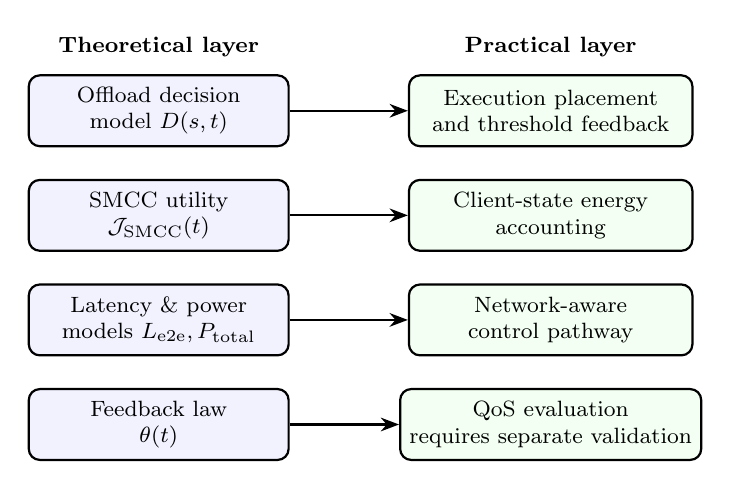
\begin{tikzpicture}[
  node distance=0.4cm and 2.0cm,
  >=Stealth,
  theory/.style={rectangle, rounded corners, draw, thick, fill=blue!5,
                 align=center, minimum width=3.3cm, minimum height=0.9cm},
  practice/.style={rectangle, rounded corners, draw, thick, fill=green!5,
                   align=center, minimum width=3.6cm, minimum height=0.9cm},
  every node/.style={font=\footnotesize}
]

% Theoretical layer (left)
\node[theory] (decision) {Offload decision\\model $D(s,t)$};
\node[theory, below=of decision] (utility) {SMCC utility\\$\mathcal{J}_{\mathrm{SMCC}}(t)$};
\node[theory, below=of utility] (models) {Latency \& power\\models $L_{\text{e2e}}, P_{\text{total}}$};
\node[theory, below=of models] (feedback) {Feedback law\\$\theta(t)$};

% Practical layer (right)
\node[practice, right=1.5cm of decision] (latency) {Execution placement\\and threshold feedback};
\node[practice, below=of latency] (energy) {Client-state energy\\accounting};
\node[practice, below=of energy] (rtt) {Network-aware\\control pathway};
\node[practice, below=of rtt] (qos) {QoS evaluation\\requires separate validation};

% Arrows: theory -> practice
\draw[->, thick] (decision) -- (latency);
\draw[->, thick] (utility) -- (energy);
\draw[->, thick] (models) -- (rtt);
\draw[->, thick] (feedback) -- (qos);

% Layer labels
\node[above=0.1cm of decision] {\textbf{Theoretical layer}};
\node[above=0.1cm of latency] {\textbf{Practical layer}};

\end{tikzpicture}
\caption{Theoretical and practical implications of NSSON: theoretical models on the left lead to measurable improvements in latency, energy, RTT, and QoS on the right.}
\label{fig:theory-practice}
\end{figure}


\subsection{Comparison with Prior Work}
Compared with SpikeNAS~\cite{putra2025spikenas}, NSSON does not incorporate Neural Architecture Search (NAS); instead, it introduces critical network orchestration and offloading mechanisms—features that remain unaddressed by the SpikeNAS framework. Compared with EC-SNN~\cite{di2024ec}, NSSON adds a feedback loop and an SDN layer that EC-SNN lacks. In contrast to conventional SDN-IoT frameworks, NSSON also supports neuromorphic simulated sensing and adaptive split computing functionalities beyond standard SDN mechanisms.  
Table~\ref{tab:comparison} in Section~\ref{sec:background}, together with the QoS results in Figs.~\ref{fig:latency_cycle}–\ref{fig:throughput_cycle}, confirms that NSSON is the sole system integrating all five dimensions of SMCC design while empirically demonstrating benefits across both compute and network metrics.

% ─── VIII. LIMITATIONS AND FUTURE WORK ────────────────────────────────────────
\section{Limitations and Future Work}
\label{sec:limitations}

\subsection{Energy-Model Uncertainty}
\label{sec:energyuncertainty}

All energy results are modeled estimates. The coefficients $W_c$, $W_t$, and $W_i$ are nominal values and do not capture DVFS, thermal throttling, workload heterogeneity, peripheral power, battery-converter losses, or device-to-device variation. A sensitivity analysis should vary each coefficient independently and report the resulting change in per-cycle energy. Physical validation requires synchronized measurements of voltage and current on the relevant Jetson Nano power rails, repeated trials, and explicit accounting for CPU, GPU, memory, network interface, and baseline idle consumption.

\subsection{Current Limitations}

\textbf{Accuracy gap in SNN}: The CNN achieved 94.84\% test accuracy, whereas the LIF-based SNN achieved 77.66\% test accuracy. This 17.18~pp disparity limits autonomous edge decision-making and motivates confidence-based offloading of low-confidence SNN outputs. Enhancing SNN performance would reduce offload frequency and potentially improve power and latency. The archived training-history files are separate training trajectories and do not constitute the evaluation records for these reported test accuracies.

\textbf{Energy validation}: The earlier Jetson Nano energy values and the reported 18\% saving are withdrawn because their units and calibration provenance were not supported by the audited artifacts. The revised formulation defines client-state energy in joules and watt-hours, but no Jetson Nano energy-saving percentage is experimentally established. The workstation GPU measurements are local GPU telemetry only and do not validate target-device energy, whole-system energy, or offloading-policy savings. Future validation should use synchronized target-device rail measurements, independent process repetitions, and explicit accounting for CPU, network-interface, and baseline power.

\subsection{Future Work}

\textbf{SpikeNAS-informed SNN design}: Applying SpikeNAS~\cite{putra2025spikenas} memory-aware NAS to the NSSON SNN sensing layer is the most promising near-term enhancement. Bridging the performance disparity from 17.18~pp to under 5~pp would significantly enhance the operational utility of the local SNN, providing a sustainable path for scaling NSSON to higher-complexity vision tasks.

\textbf{Real Jetson Nano deployment}: Running NSSON on actual Jetson Nano hardware would enable ground-truth measurement of the power model, and it would allow for the validation of the latency decomposition under authentic hardware and thermal constraints.\revblue{Although the current implementation is evaluated within a
Mininet-WiFi emulation, all NSSON components are designed to map
directly onto real deployments: the neuromorphic sensing plane runs on
Jetson Nano-compatible PyTorch/SpikingJelly code, the telemetry bus uses
filesystem-based logs or could be replaced by a message queue such as
MQTT, and the Ryu controller operates identically on physical OpenFlow
switches and wireless access points. The only emulation-specific aspects
are the Mininet-WiFi topology description and link parameter settings,
which can be instantiated on commodity SDN-enabled hardware without
changing the control logic.}

\textbf{Multi-AP mobile topology}: Scaling the Mininet-WiFi topology to support mobile stations and multiple access points would empower the Ryu controller to run proactive handover management. This extension is important for validation for NSSON's ability to dynamically re-route offloading traffic based on real-time signal strength and AP load.

% ─── IX. CONCLUSION ───────────────────────────────────────────────────────────
\subsection*{Data and Code Availability}
The reproducibility artifacts include training histories, inference-decision logs, latency and energy telemetry, Ryu flow-installation logs, topology and controller configuration, plotting scripts, and the generated figures. These artifacts allow independent verification of the reported sensing results, threshold sweep, modeled-energy calculations, and SDN flow-association behavior.

\section{Conclusion}
\label{sec:conclusion}

This paper presented NSSON as an SDN-oriented SMCC framework
connecting CNN/SNN sensing, shared telemetry, confidence-based
execution placement, threshold feedback, and programmable
network control. The revised evaluation separates the scope of
each experiment and distinguishes proposed architectural
capabilities from directly demonstrated behavior.

The audited network-emulation experiments execute actual model
inference between namespaces on one workstation. They contain
300 requests per policy in each of three repetitions and support
application-level client--server identity matching and causal
threshold updates. Increasing the threshold increases offloading
under the rule $C(s)<\theta(t)$ for a fixed confidence trace.
The accuracy-aware controller evaluated here is oracle-only
because it consumes ground-truth labels. Energy feedback was
disabled in these experiments.

The corrected energy accounting distinguishes watts, joules,
and watt-hours. Separate workstation GPU telemetry gives
amortized energies of $0.066159 \pm 0.002913$~J per completed
CNN inference and $0.734507 \pm 0.022852$~J per completed
SNASNet SNN inference, expressed as means and sample standard
deviations across three workload blocks within one process.
The evaluated SNN did not exhibit an energy advantage over the
CNN on this GPU. These measurements exclude CPU, network-interface,
and whole-system energy and do not validate Jetson Nano energy
or an offloading-energy-saving percentage.

Application-level identity matching must not be equated with
PacketIn-to-OpenFlow association. Similarly, static-forwarding
inference experiments do not establish inference-aware Ryu
orchestration, queue differentiation, or SLA enforcement.
Those capabilities require separately documented implementation
and experimental evidence. Future work includes target-device
power measurement, independent-process energy repetitions,
and validation of cross-layer control under concurrent traffic.

\bibliographystyle{IEEEtran}
\bibliography{references}

\end{document}
